\appendix

\section{Appendix: Användartester}

\subsection{SUS-formulär}

\begin{figure}[H]
  \centering
  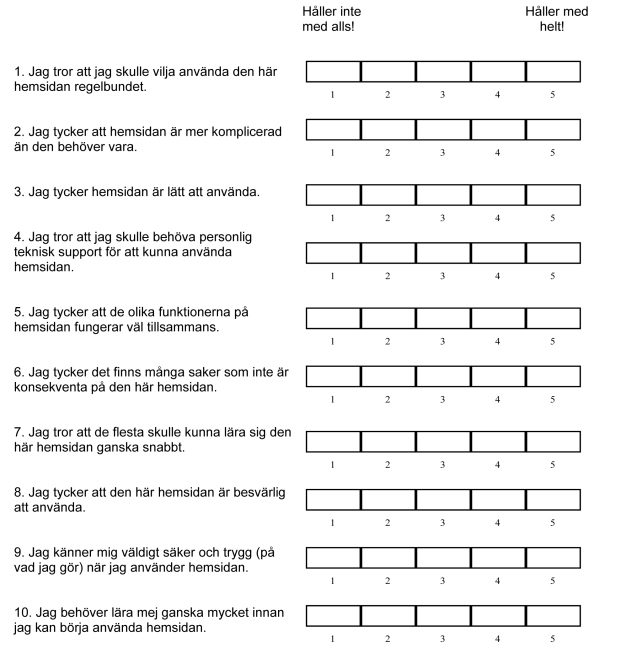
\includegraphics[width=0.75\textwidth]{bilaga/sus/form.jpg}
  \caption{SUS-formuläret vi använde}
\end{figure}

\subsection{SUS-resultat}

\begin{figure}[H]
  \centering
  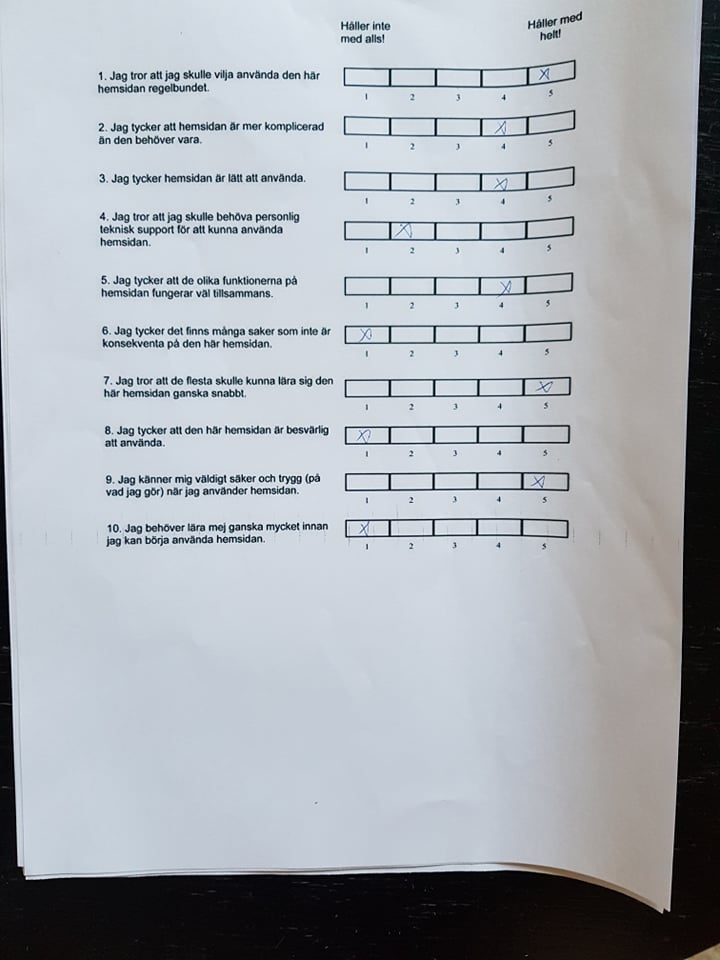
\includegraphics[width=0.75\textwidth]{bilaga/sus/ps1.jpg}
  \caption{Person 1}
\end{figure}

\begin{figure}[H]
  \centering
  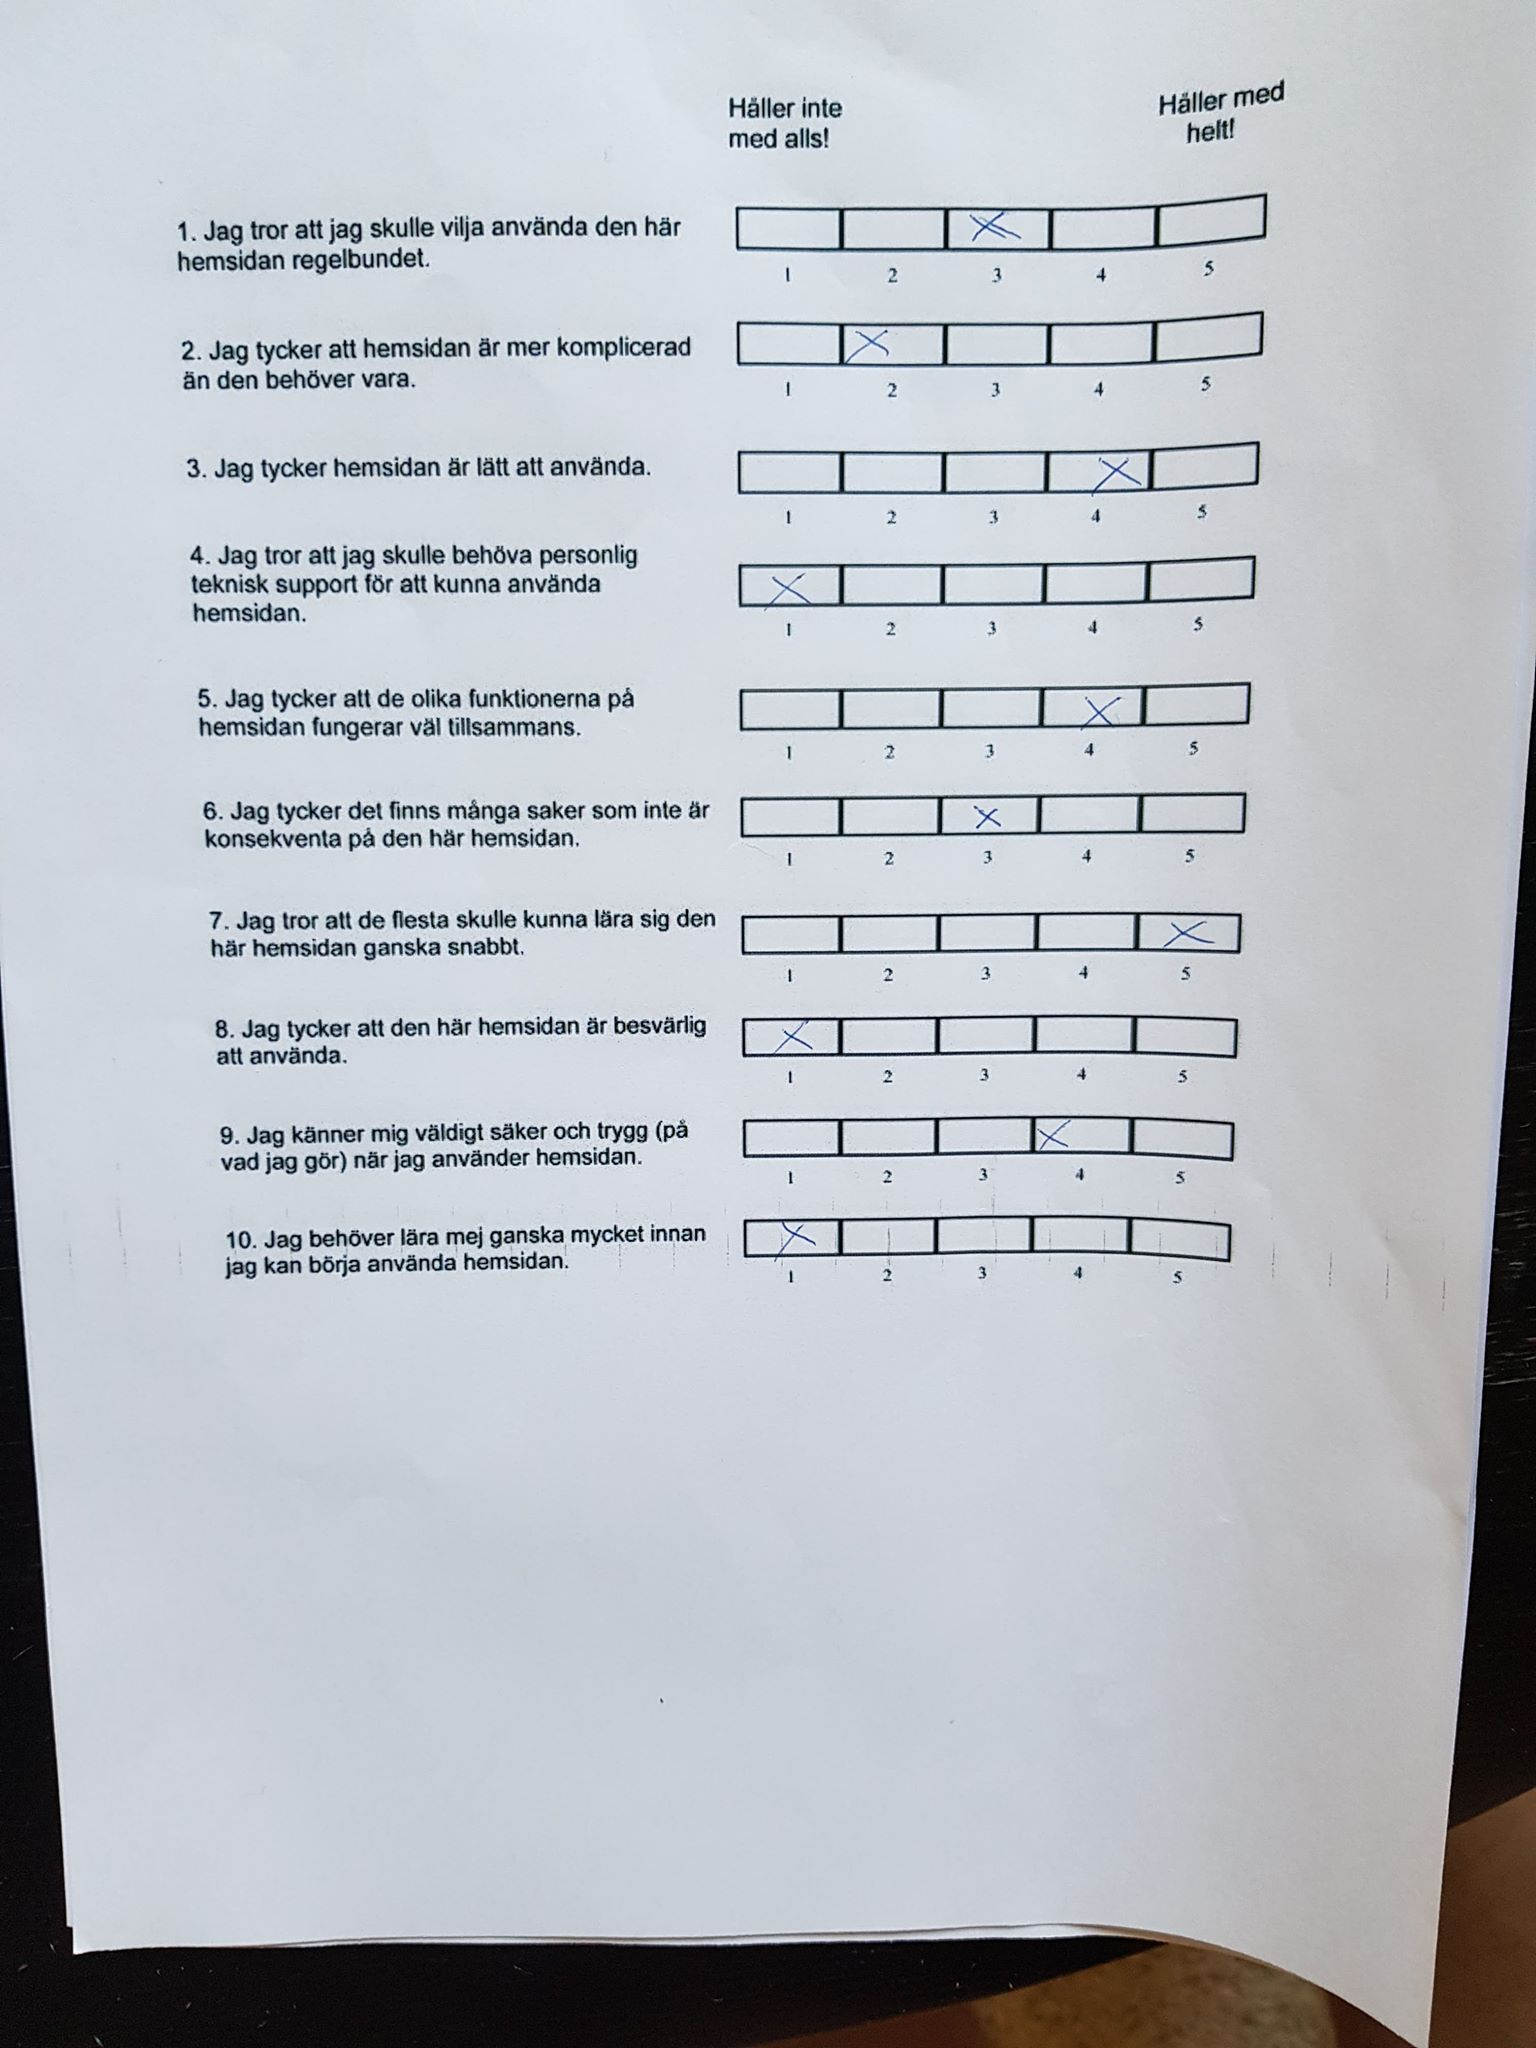
\includegraphics[width=0.75\textwidth]{bilaga/sus/ps2.jpg}
  \caption{Person 2}
\end{figure}

\begin{figure}[H]
  \centering
  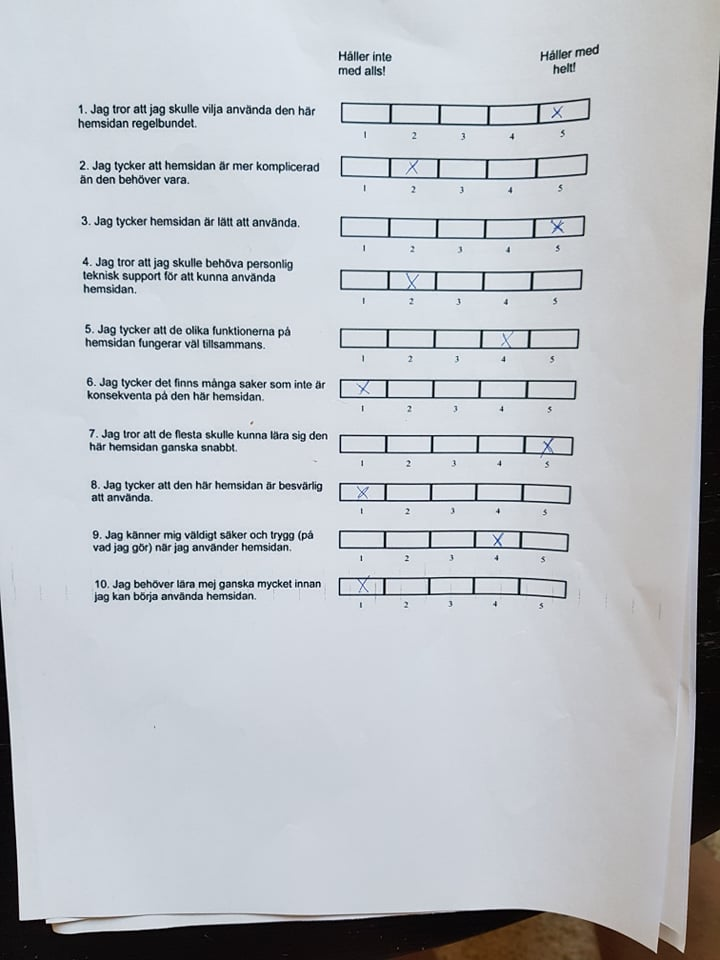
\includegraphics[width=0.75\textwidth]{bilaga/sus/ps3.jpg}
  \caption{Person 3}
\end{figure}

\begin{figure}[H]
  \centering
  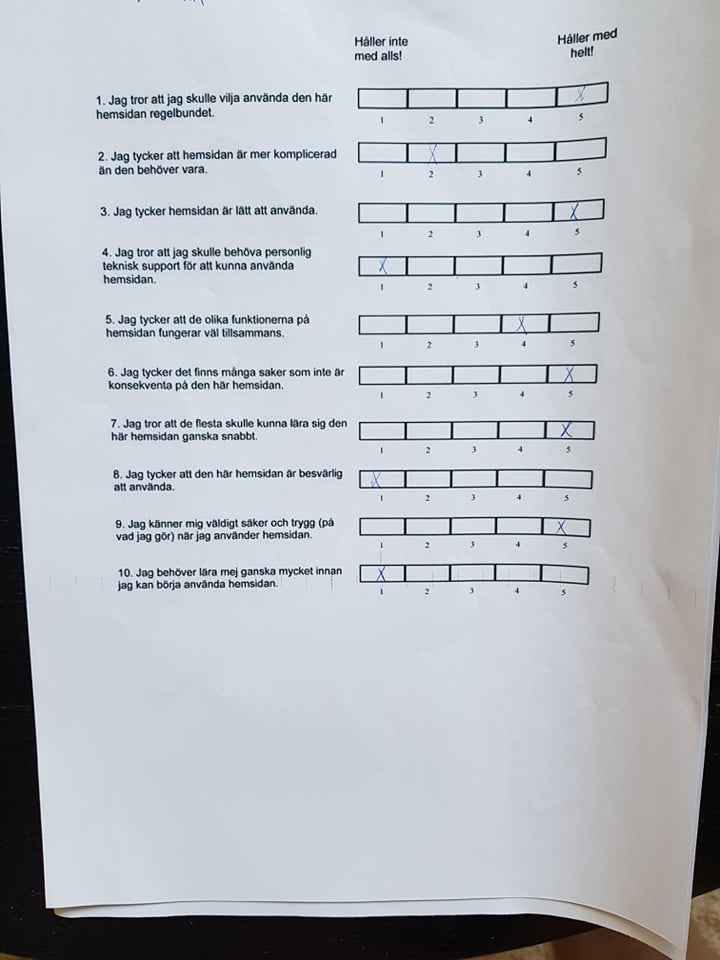
\includegraphics[width=0.75\textwidth]{bilaga/sus/ps4.jpg}
  \caption{Person 4}
\end{figure}

\begin{figure}[H]
  \centering
  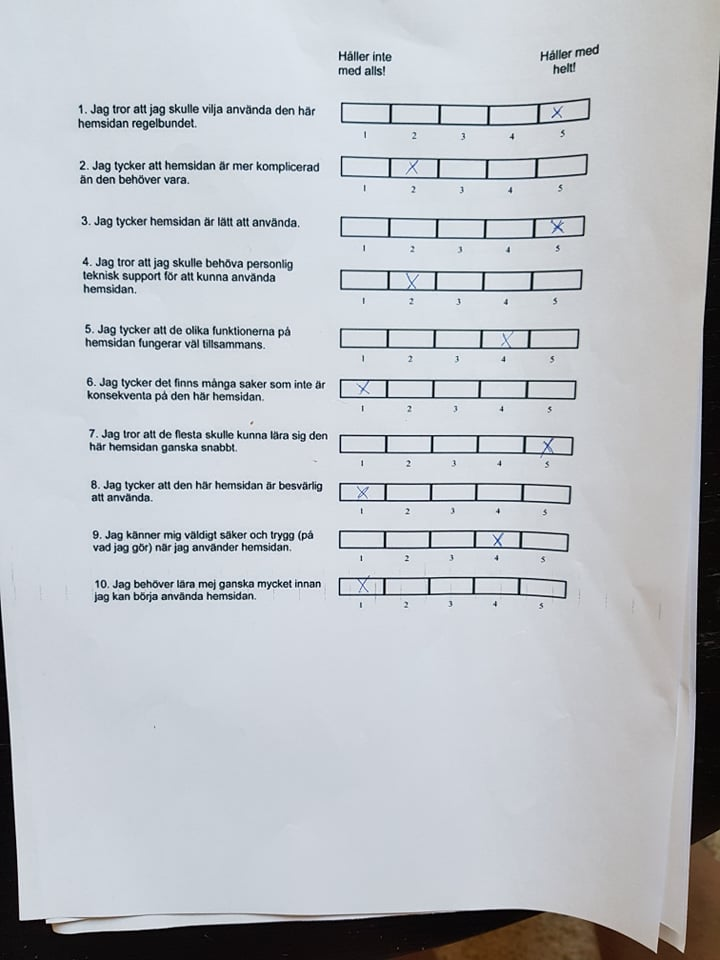
\includegraphics[width=0.75\textwidth]{bilaga/sus/ps5.jpg}
  \caption{Person 5}
\end{figure}

\subsection{Intervjusvar}

\textbf{Frågor}:
\begin{enumerate}
\item Var rättningsförslagen tydliga eller var det något specifikt du inte förstod?
\item Är det något i processen att lämna in en rapport som är oklart?
\item Finns det något du saknar med applikationen?
\item Tyckte du något var särskilt bra med applikationen, i så fall vad?
\item Tyckte du något var dåligt med applikationen, i så fall vad?
\end{enumerate}

\textbf{Person 1}:
\begin{enumerate}
\item Det var tydligt även om det var första gången. En genomgång hade dock behövts.
\item Sparningen var kanske något oklart.
\item Inget på rak arm.
\item Att man kunde se var felen fanns, att det var markerat. Gick snabbt. Att det angavs sig var rubrikerna skulle ligga.
\item Inte som han kunde se. Att allt blir rättat är viktigt, finns dock fel risk att folk skriver slarvigt första gången. Annars tummar upp.
\end{enumerate}

\textbf{Person 2}:
\begin{enumerate}
\item Att citat-varningarna kommer i två felmeddelanden.
\item Kanske om han var själv, men efter första hjälpen kan ha klara det hädanefter.
\item Nej inte direkt, förslagen är bra.
\item När man trycker så highlightas felen. Gjorde det väldigt enkelt. Kanske kan man markera geografisk plats än att enbart markera rubriken.
\item Nej.
\end{enumerate}

\textbf{Person 3}:
\begin{enumerate}
\item Nej, det står vad som ska ändras. Och vart de ska ändras.
\item Nej.
\item Inte som han kan på.
\item Citattecken-varningar.
\item Nej.
\end{enumerate}

\textbf{Person 4}:
\begin{enumerate}
\item De var tydliga, stod var det.
\item Nej, det var smidigt.
\item Hade velat ändra direkt på sidan.
\item Kan vara ett jättestort hjälp till de som inte tycker att det är roligt att skriva. Kan vara bra att hitta talspråksfel.
\item Nej.
\end{enumerate}

\textbf{Person 5}:
\begin{enumerate}
\item Man bör kunna slå ihop förbjudna ord. Motivera kanske varför man inte ska använda gammeldags ord. Man ska kunna copy-pastea.
\item Det är ganska rakt fram. Man skulle vilja rangordna felen utifrån var de är i dokumentet, eller kanske utifrån i “allvarlighetsgraden”. Kanske kan använda olikafärger för att gradera. När man klickar på ett felmeddelande så går sidan direkt till felet.
\item Nej inget direkt, känns ganska simpelt.
\item Att hitta alla fel.
\item Copy-paste-funktionen som saknas.
\end{enumerate}

\section{Appendix: Applikationen}

\subsection{Polisrelaterade ord}

\section{Appendix: Polisrapporter}\label{b:rapporter}

\begin{figure}[H]
  \centering
  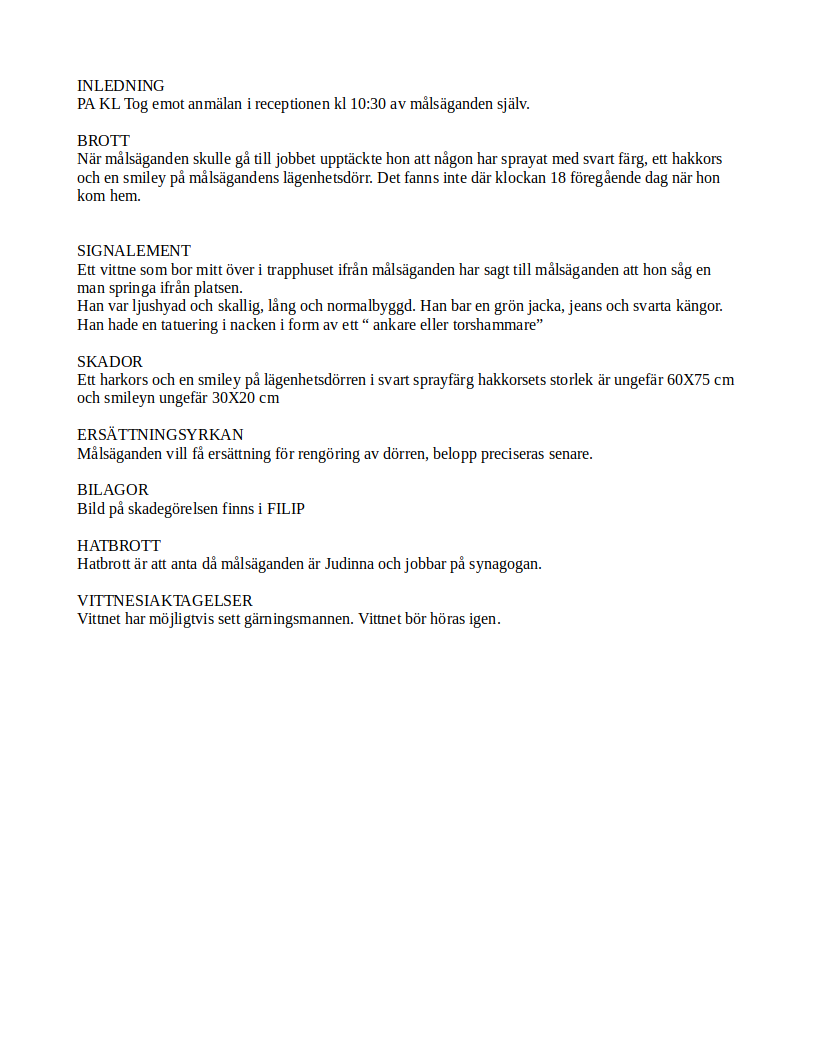
\includegraphics[width=0.75\textwidth]{bilaga/rapporter/r1.png}
  \caption{Rapport 1}
\end{figure}

\begin{figure}[H]
  \centering
  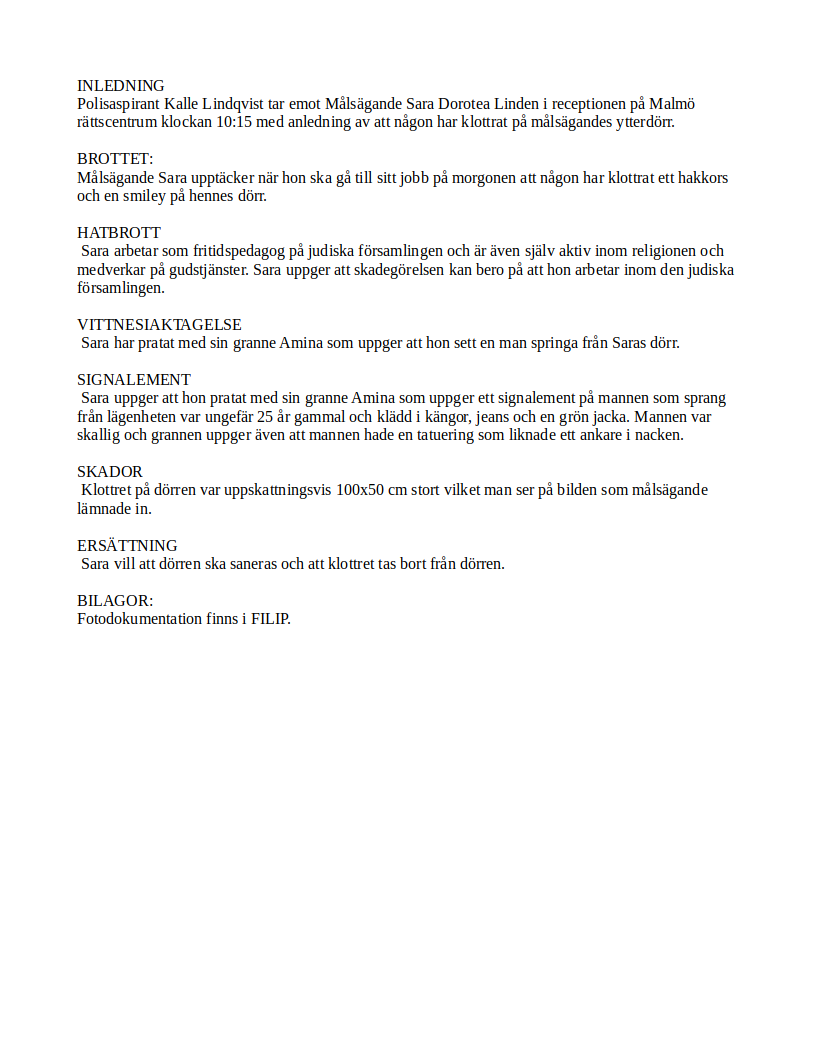
\includegraphics[width=0.75\textwidth]{bilaga/rapporter/r2.png}
  \caption{Rapport 2}
\end{figure}

\begin{figure}[H]
  \centering
  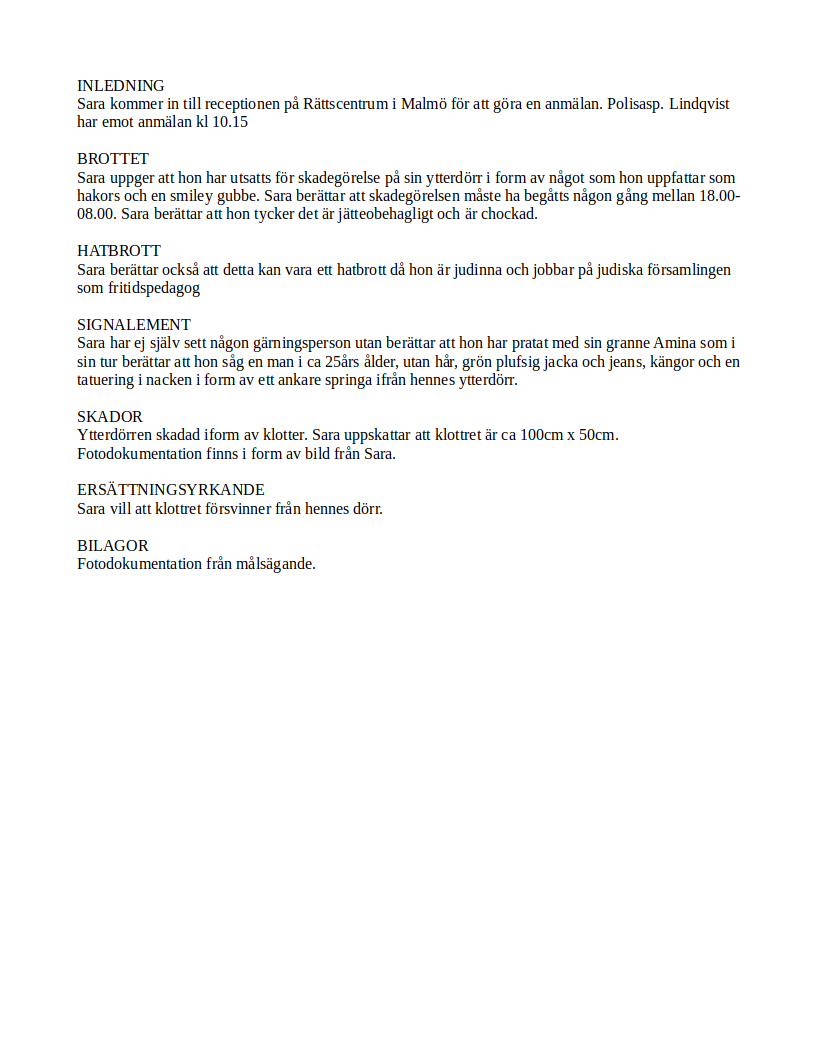
\includegraphics[width=0.75\textwidth]{bilaga/rapporter/r3.png}
  \caption{Rapport 3}
\end{figure}

\begin{figure}[H]
  \centering
  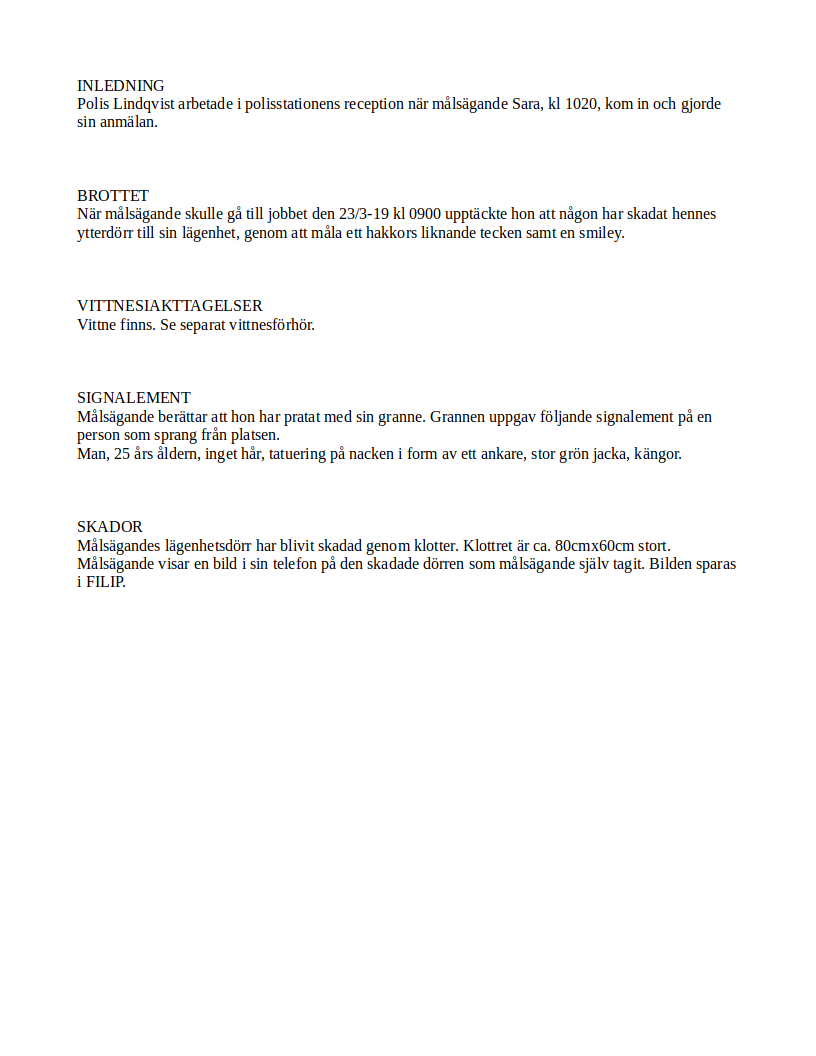
\includegraphics[width=0.75\textwidth]{bilaga/rapporter/r4.png}
  \caption{Rapport 4}
\end{figure}

\begin{figure}[H]
  \centering
  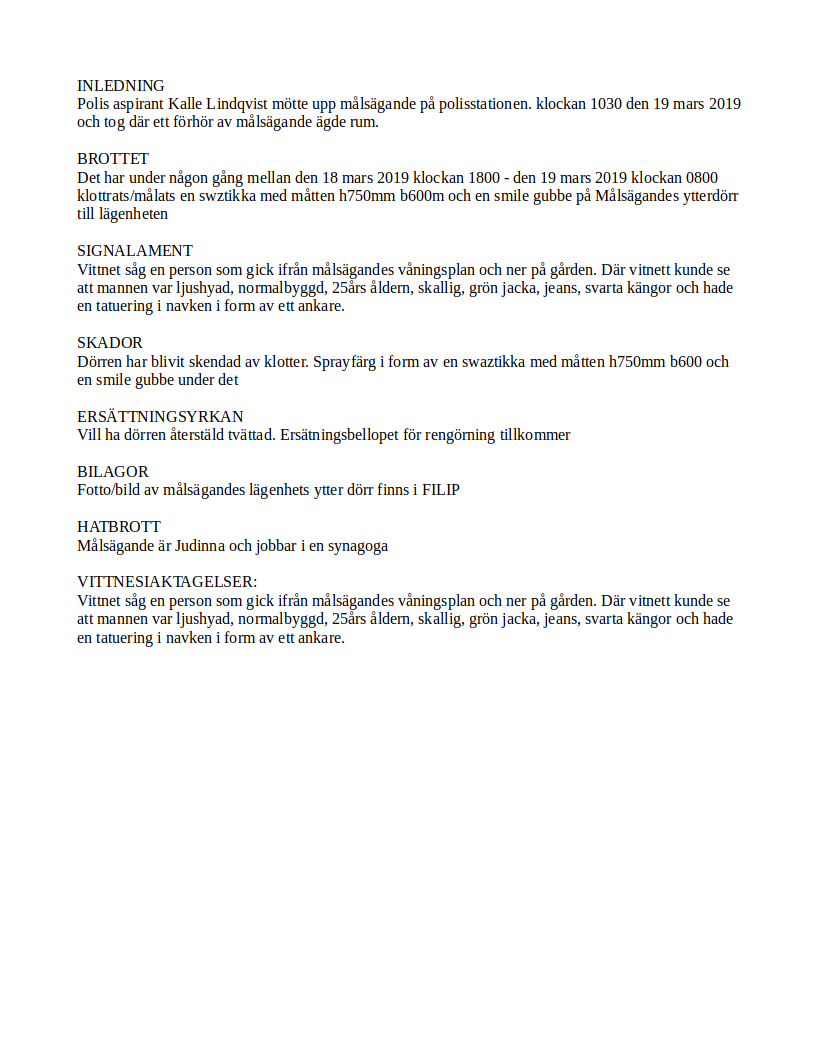
\includegraphics[width=0.75\textwidth]{bilaga/rapporter/r5.png}
  \caption{Rapport 5}
\end{figure}

\begin{figure}[H]
  \centering
  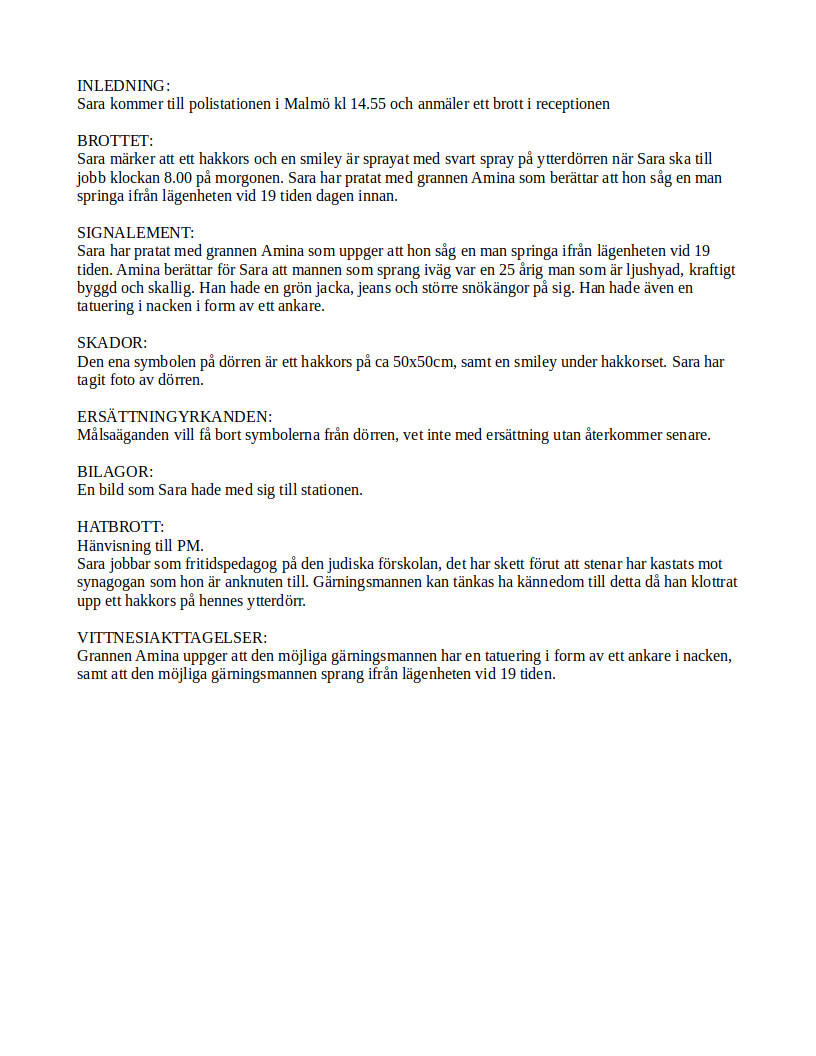
\includegraphics[width=0.75\textwidth]{bilaga/rapporter/r6.png}
  \caption{Rapport 6}
\end{figure}

\begin{figure}[H]
  \centering
  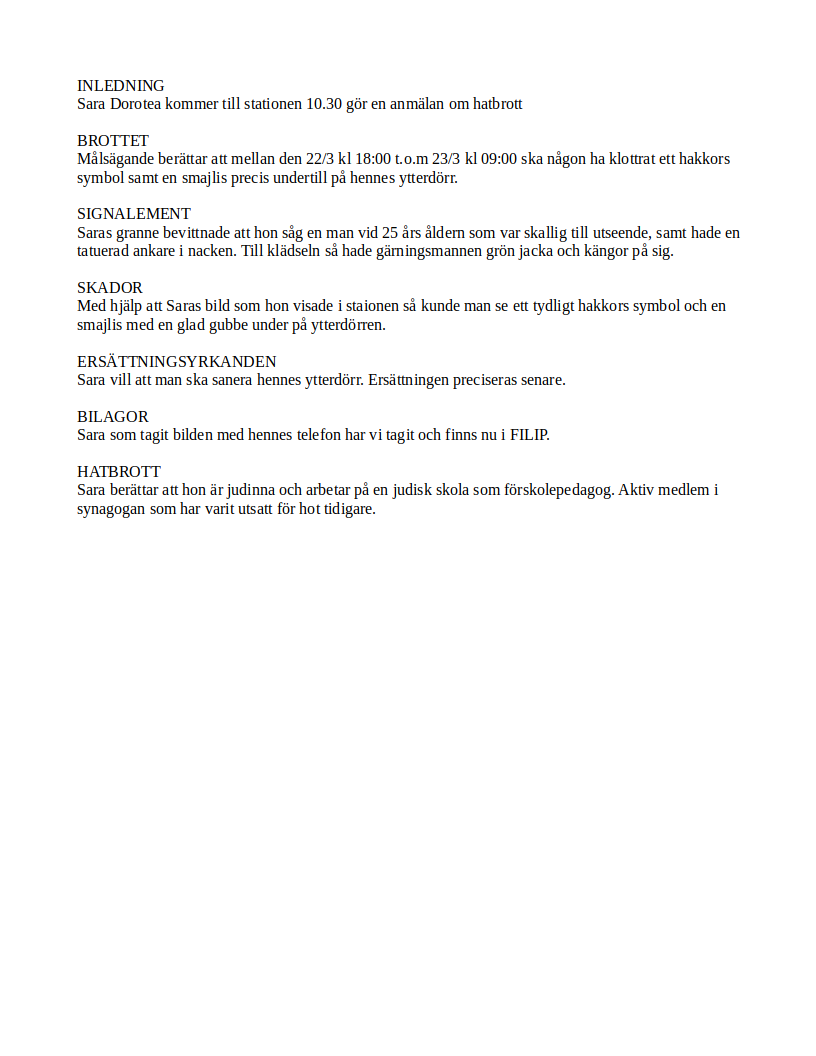
\includegraphics[width=0.75\textwidth]{bilaga/rapporter/r7.png}
  \caption{Rapport 7}
\end{figure}

\begin{figure}[H]
  \centering
  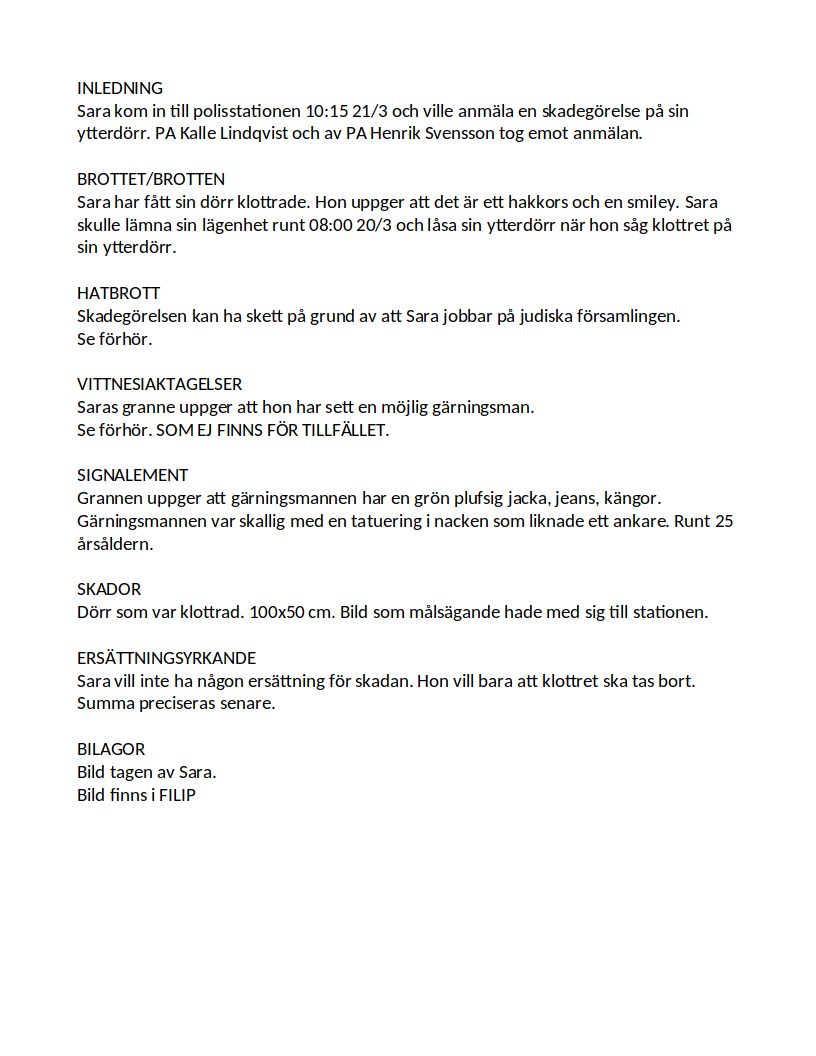
\includegraphics[width=0.75\textwidth]{bilaga/rapporter/r8.png}
  \caption{Rapport 8}
\end{figure}

\begin{figure}[H]
  \centering
  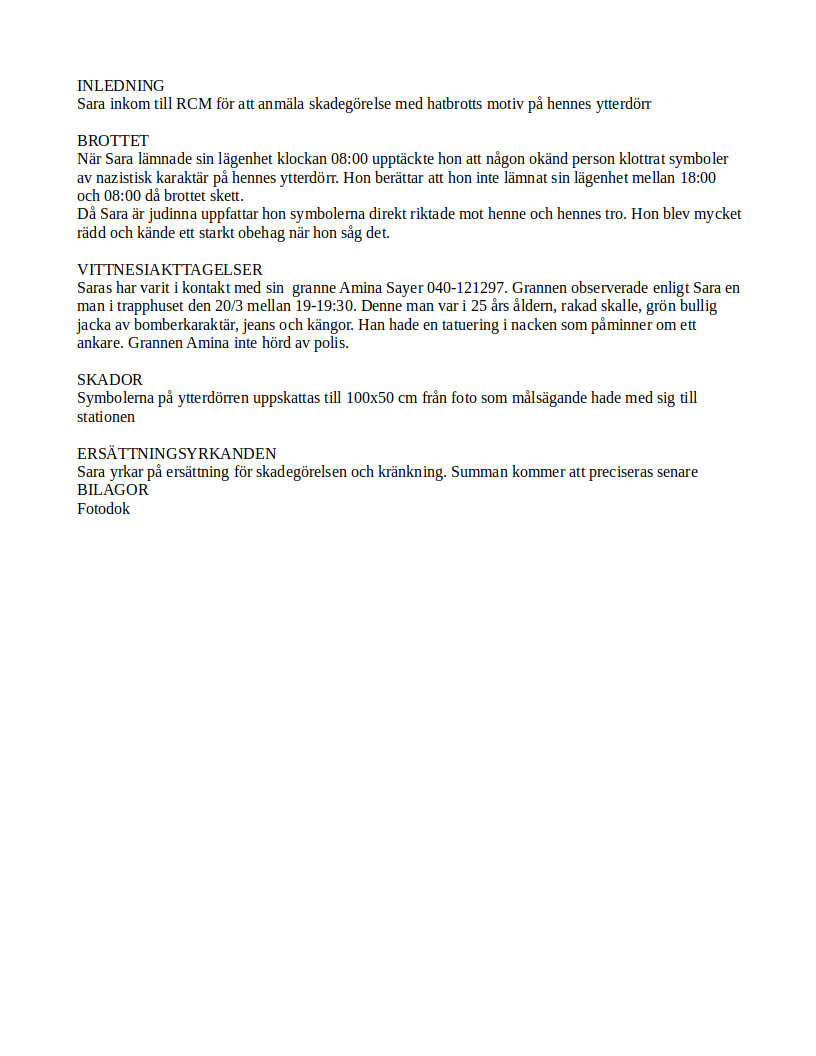
\includegraphics[width=0.75\textwidth]{bilaga/rapporter/r9.png}
  \caption{Rapport 9}
\end{figure}

\begin{figure}[H]
  \centering
  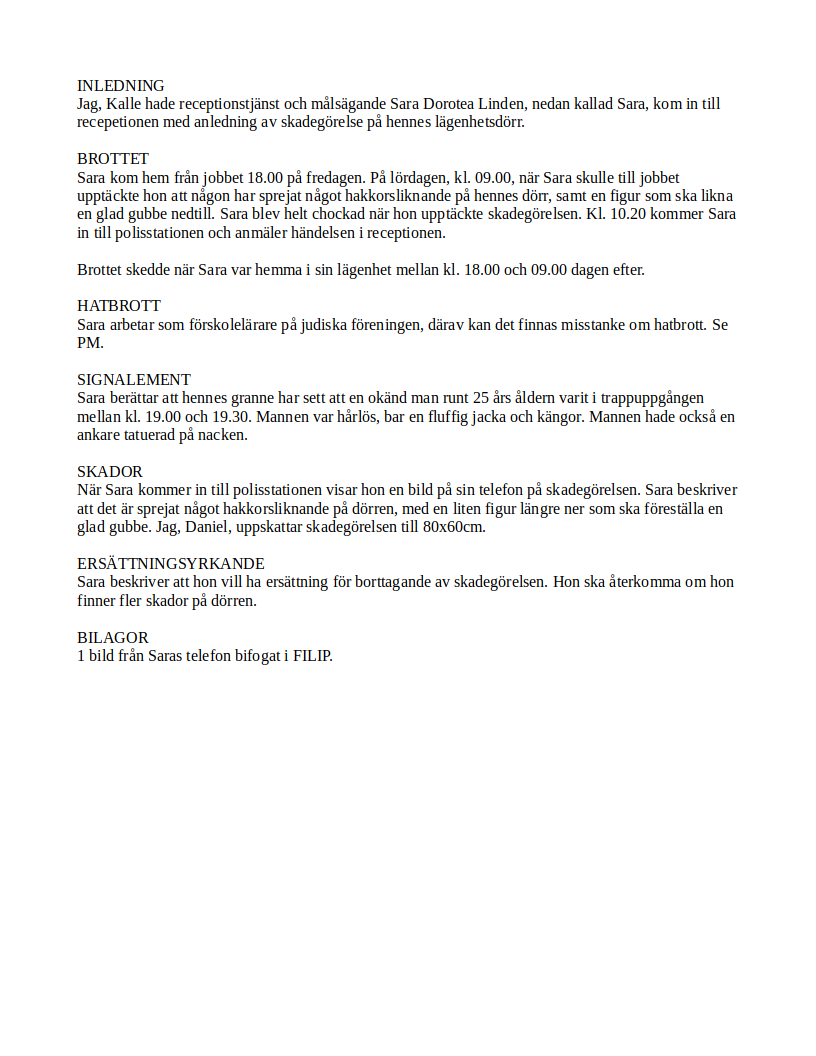
\includegraphics[width=0.75\textwidth]{bilaga/rapporter/r10.png}
  \caption{Rapport 10}
\end{figure}

\begin{figure}[H]
  \centering
  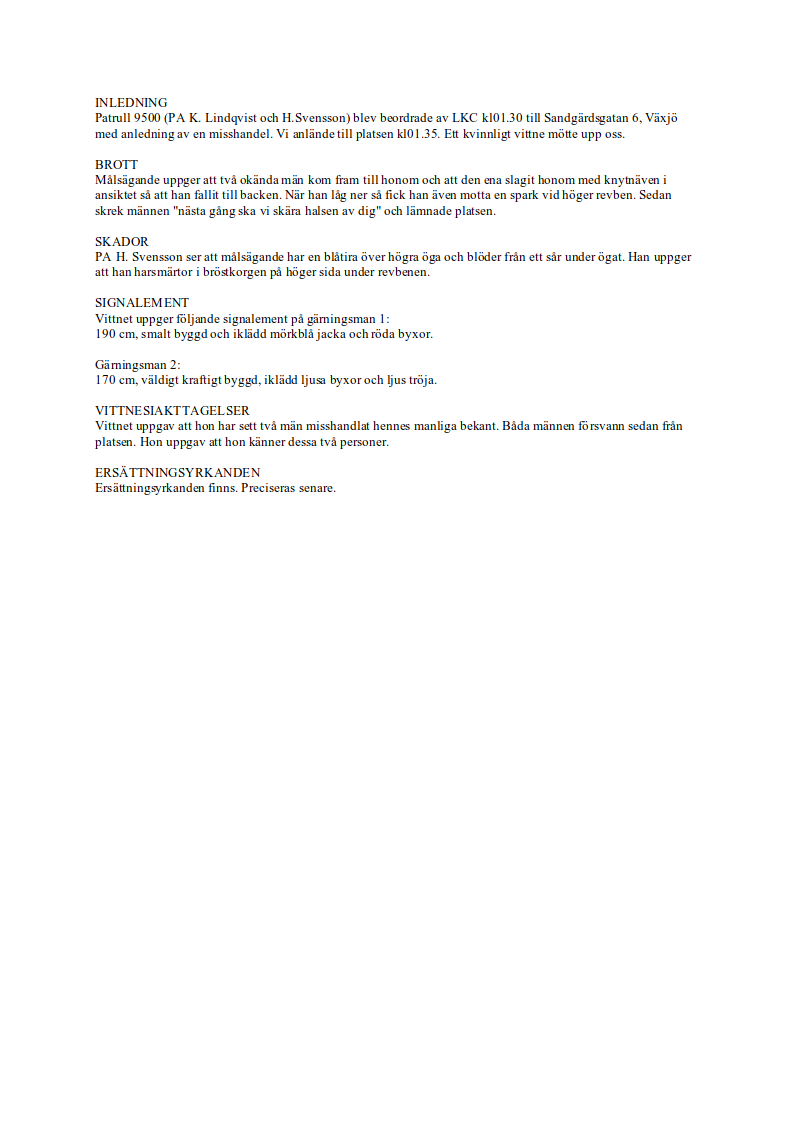
\includegraphics[width=0.75\textwidth]{bilaga/rapporter/r11.png}
  \caption{Rapport 11}
\end{figure}

\begin{figure}[H]
  \centering
  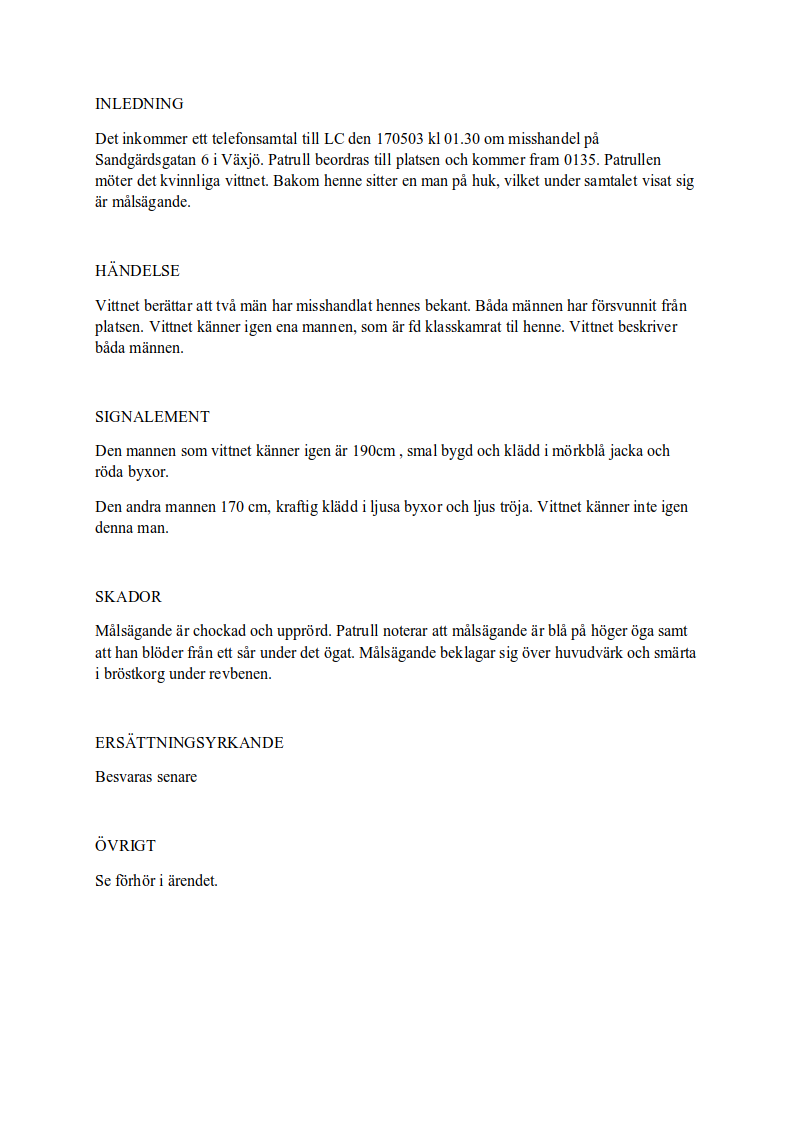
\includegraphics[width=0.75\textwidth]{bilaga/rapporter/r12.png}
  \caption{Rapport 12}
\end{figure}

\begin{figure}[H]
  \centering
  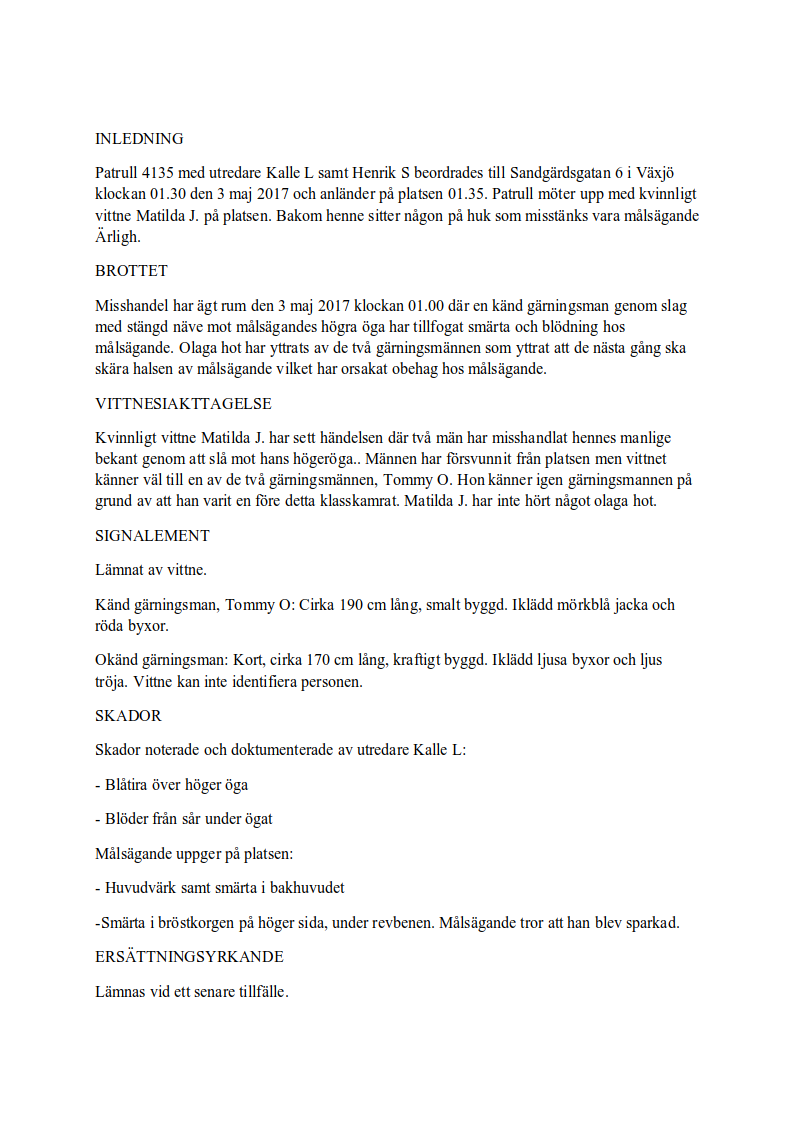
\includegraphics[width=0.75\textwidth]{bilaga/rapporter/r13.png}
  \caption{Rapport 13}
\end{figure}

\begin{figure}[H]
  \centering
  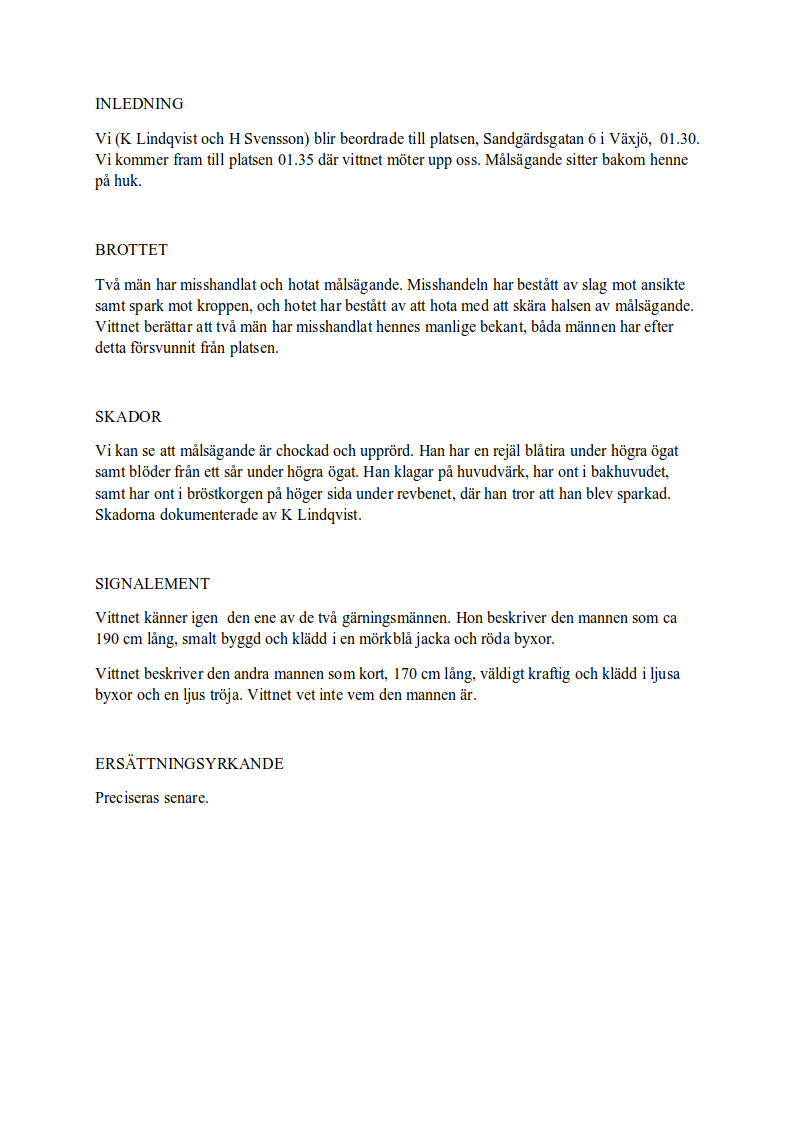
\includegraphics[width=0.75\textwidth]{bilaga/rapporter/r14.png}
  \caption{Rapport 14}
\end{figure}

\begin{figure}[H]
  \centering
  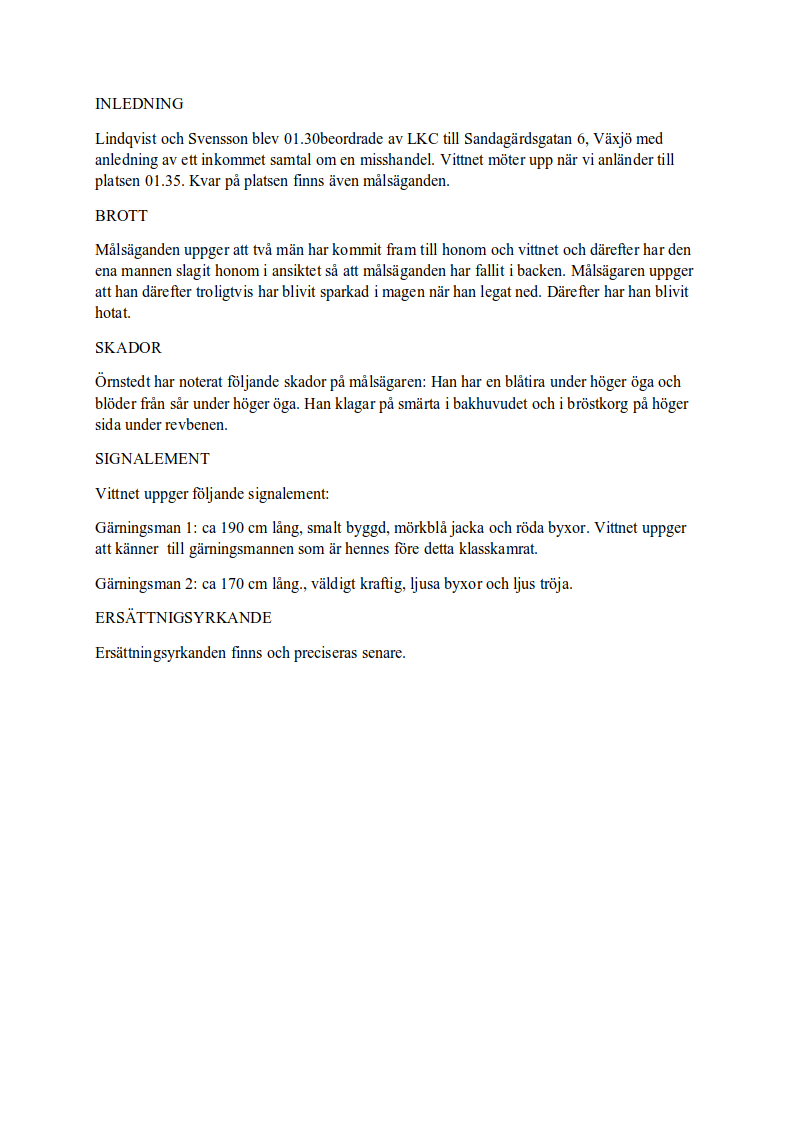
\includegraphics[width=0.75\textwidth]{bilaga/rapporter/r15.png}
  \caption{Rapport 15}
\end{figure}

\begin{figure}[H]
  \centering
  
\includegraphics[width=0.75\textwidth]{bilaga/rapporter/r16.png}
  \caption{Rapport 16}
\end{figure}

\begin{figure}[H]
  \centering
  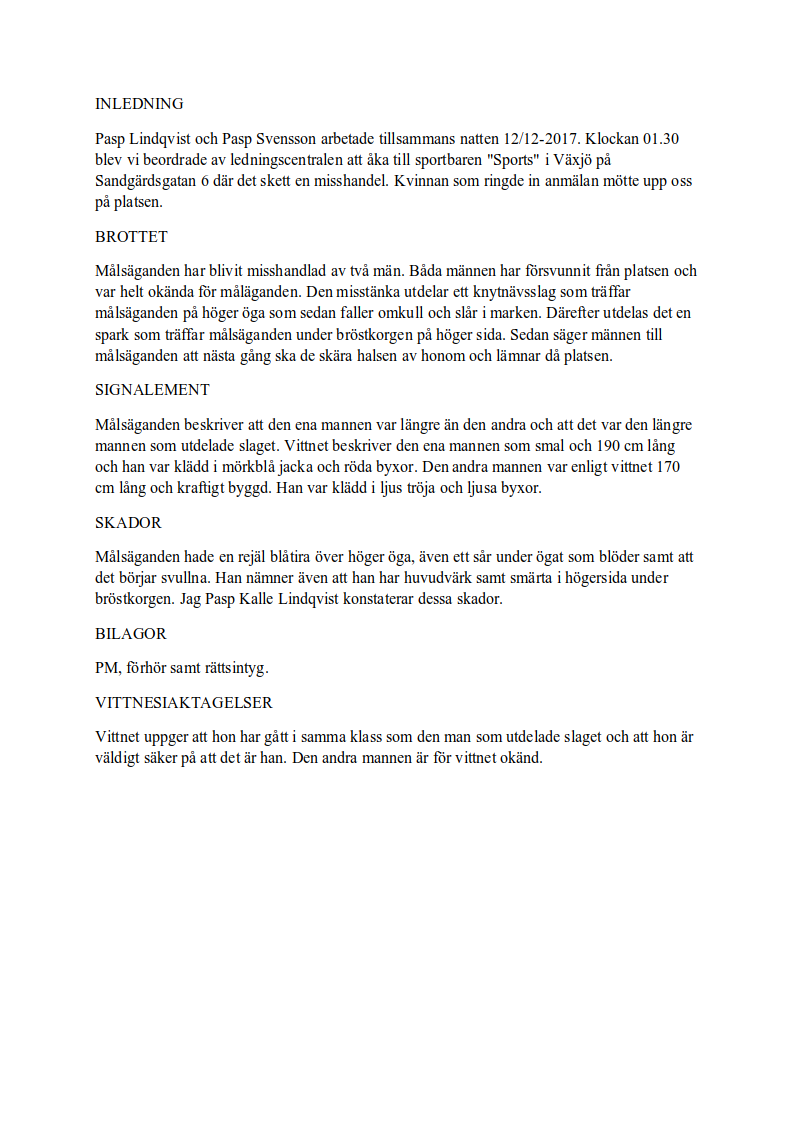
\includegraphics[width=0.75\textwidth]{bilaga/rapporter/r17.png}
  \caption{Rapport 17}
\end{figure}

\begin{figure}[H]
  \centering
  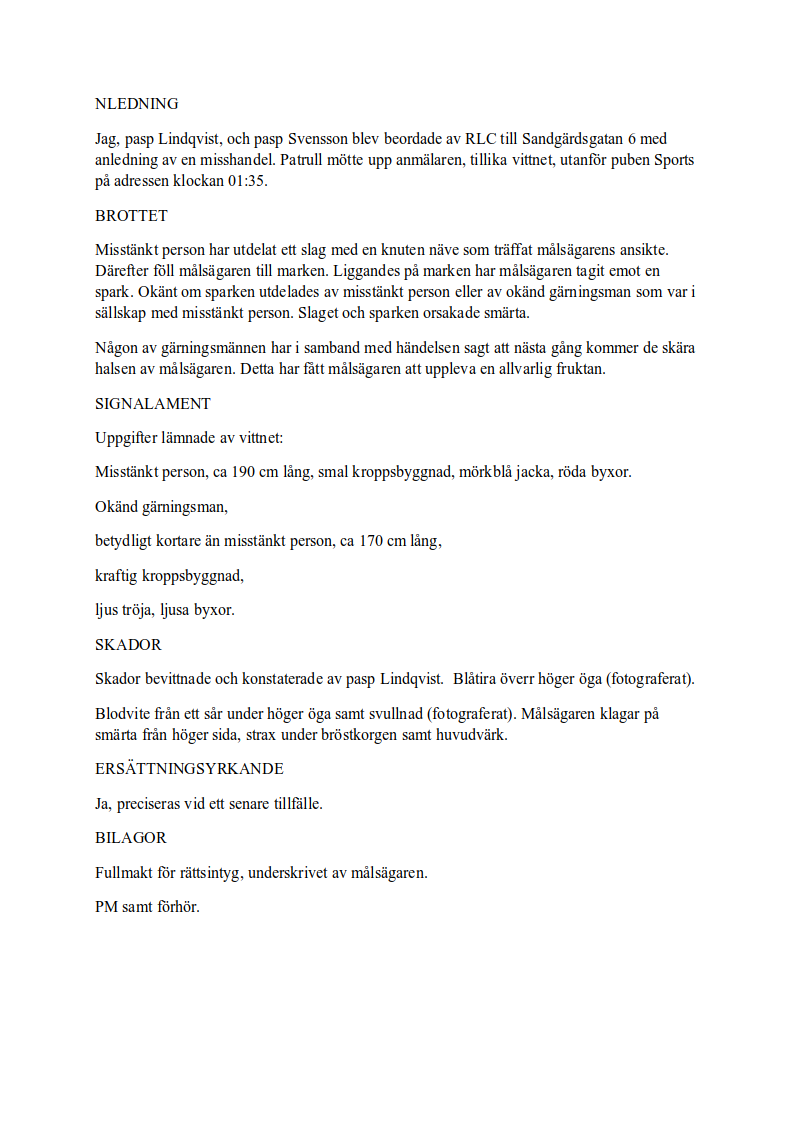
\includegraphics[width=0.75\textwidth]{bilaga/rapporter/r18.png}
  \caption{Rapport 18}
\end{figure}

\begin{figure}[H]
  \centering
  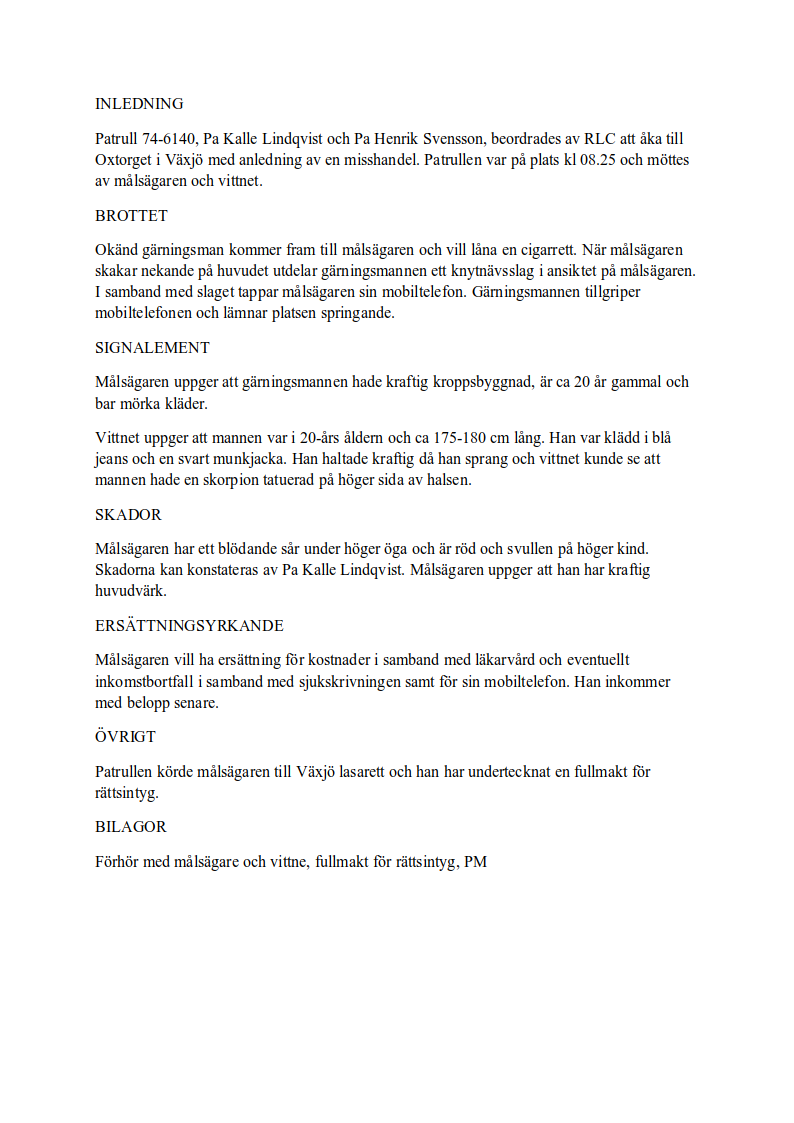
\includegraphics[width=0.75\textwidth]{bilaga/rapporter/r19.png}
  \caption{Rapport 19}
\end{figure}

\begin{figure}[H]
  \centering
  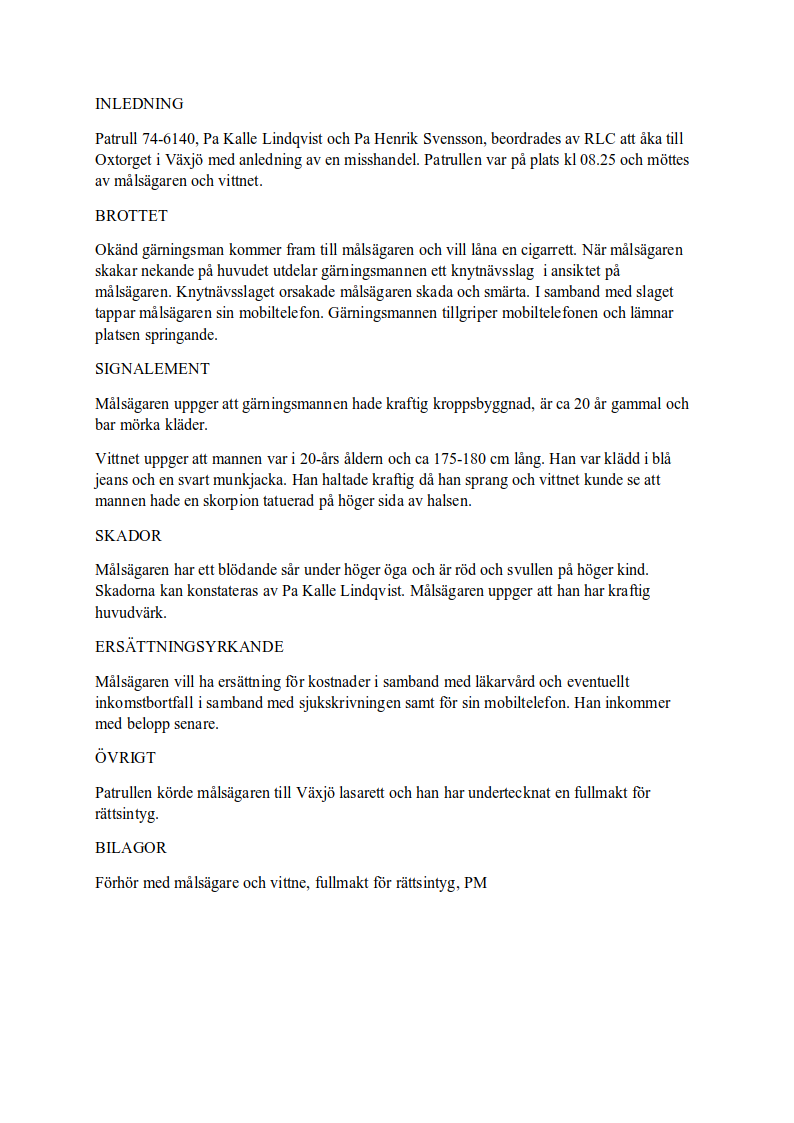
\includegraphics[width=0.75\textwidth]{bilaga/rapporter/r20.png}
  \caption{Rapport 20}
\end{figure}